\documentclass[12pt]{article}
\usepackage{indentfirst}
\usepackage[ipaex]{pxchfon}
\usepackage{geometry}
\usepackage[dvipdfmx]{graphicx}
\usepackage{threeparttable}
\usepackage{amsmath}
\usepackage{amssymb}
\usepackage{bm}
\usepackage{url}
\usepackage{float}
\usepackage{geometry}
\usepackage{array}
\usepackage{booktabs}
\usepackage{setspace}
\usepackage{array}
\usepackage{graphicx}
\usepackage{eurosym}
\makeatletter
\newdimen\arrayrulewidthb
\arrayrulewidthb=\p@\relax
\newcolumntype{I}{!{\vrule width \arrayrulewidthb}}
\def\hlineb{
    \noalign{\ifnum0=`}\fi\hrule \@height \arrayrulewidthb \futurelet
        \reserved@a\@xhlineb}
    \def\@xhlineb{\ifx\reserved@a\hlineb
            \vskip\doublerulesep
            \vskip-\arrayrulewidthb
        \fi
        \ifnum0=`{\fi}}
\makeatother

\setstretch{1.63}
\setlength{\topmargin}{4.6truemm}
%\setlength{\textheight}{480pt}
\setlength{\textheight}{29\baselineskip}
\addtolength{\textheight}{\topskip}

\setlength{\textwidth}{40zw}
\setlength{\oddsidemargin}{1cm}
\setlength{\evensidemargin}{1cm}
\setcounter{tocdepth}{2}
\geometry{left=20mm,right=20mm,top=30mm,bottom=30mm}

\title{\LARGE{An positive analysis of the monetary \\ spillover channels in Europe and Japan}
    %主題
    \\ \vspace{\baselineskip}
    \Large{Faculty of Economics, Kyoto University \\} %副題
}

\author{
    Senna Ohmura
}

\date{
    \ \\
    \ \\
    \ \\
    \ \\
    November 2020}

\begin{document}
\maketitle
\thispagestyle{empty} % 表紙にページ数を入れない
\newpage
\thispagestyle{empty} % 概要にページ数をつけない

\addcontentsline{doc}{section}{Abstract}
\abstract{
    The purpose of this paper is to identify the spillover channels of monetary easing policies in Europe and Japan today.
    In addition, I suggest what kind of additional monetary easing might work more effectively.
    To this end, I use macroeconomic data for Europe and Japan to analyze how monetary easing policies affect financial markets,
    foreign exchange markets, and inflation rates in these regions.

    \vspace{110pt}

    I would like to thank Mr. Yasushi Harada (former member of the Policy Board of the Bank of Japan), Mr. Takekazu Iwamoto (former professor at the Graduate School of Economics, Kyoto University), and many others for their helpful and enthusiastic comments on this paper.
    I would like to express my gratitude to them.
    However, the responsibility for any possible errors or assertions in this paper goes without saying to the author.}

\newpage
\thispagestyle{empty}
\pagenumbering{roman} % 目次のページをローマ数字に 
\tableofcontents % 目次の挿入
\newpage
\pagenumbering{arabic} % ページ数をアラビア数字に

\section{Introduction}

The subprime loan problem in the U.S. triggered the Lehman Shock in 2008, which led to a global deflationary trend in many countries.
In response, the central banks of each country implemented monetary easing policies to purchase government bonds and other assets from the financial markets and lowered their policy interest rates.
As a result, the balance sheets of central banks expanded rapidly and policy interest rates became extremely low.
The effects of this quantitative monetary easing policy can be explained in the following four points.

\begin{enumerate}
    \setlength{\leftskip}{30pt}
    \item The expansion of the monetary base will raise inflation expectations.
    \item The expectation of a prolonged period of low interest rates lowers long-term interest rates and brings about a booming economy.\\(Policy Duration Effect)
    \item Under zero or negative interest rates, the buildup of current account balances at the central bank causes financial institutions to restructure their portfolios and increase their lending.\\(Portfolio Rebalancing Effect)
    \item As domestic interest rates fall, capital flows out of the country, depreciating the local currency.
    \item Asset prices (stock prices, real estate prices) rise as expectations of future price increases increase.\\ (Forward-Looking Expectation Formation)
\end{enumerate}

The Policy Duration Effect is caused by future expectations and occurs when the central bank makes an announcement that it will continue its monetary easing policy until certain conditions are met.
When the central bank announces that it will continue its monetary easing policy until certain conditions are met, the market's expectation of future short-term interest rates declines, and the current long-term interest rate declines accordingly.

the Portfolio Rebalancing Effect means that when funds are supplied to financial institutions and the excess reserves in the current account of the central bank are at zero or negative interest rates, financial institutions will reconfigure their portfolios,
and as a result, excess funds will be used for market operations and loans.
Specifically, an increase in lending leads to an expansion of capital investment, and an increase in the purchase of foreign bonds leads to a depreciation of the local currency.

In Japan, the Bank of Japan (BOJ) implemented the "Comprehensive Monetary Easing Policy" since October 2010, which includes the restoration of the zero interest rate policy and the establishment of a fund for asset purchases, etc.
The price stability target of 2\% was introduced in January 2013, and the "Quantitative and Qualitative Easing (QQE) Policy" was launched in April 2013. This led to a sharp increase in the monetary base.
This led to a rapid expansion of the monetary base and a commitment to the 2\% inflation target.
In addition, in February 2016, the BOJ launched "Quantitative and Qualitative Monetary Easing with Negative Interest Rates," in which a negative interest rate of -0.1\% was applied to excess reserves in the BOJ's current account, suggesting the possibility of deeper easing in the future.
In September 2016, the BOJ started "Quantitative and Qualitative Monetary Easing with Long and Short Term Interest Rate Operations", which includes "yield curve control" and "overshooting commitments", but the interest rate on excess reserves in the BOJ's current account remains unchanged at -0.1\%.

In Europe, the European Central Bank (ECB) introduced the Securities Markets Programme (SMP) in May 2010 in response to the Greek crisis that erupted in 2009.
In June 2014, a negative interest rate of -0.1\% was introduced for the central bank's deposit rate (facility rate), and in March 2015, the ECB launched a full-fledged quantitative easing policy.
The ECB has now deepened the central bank deposit rate to -0.5\%, which is a larger scale of easing than in Japan.
On the other hand, the "Quantitative Definition of Price Stability," which sets the inflation target at a level below but close to 2\%, has remained unchanged for a long time since its definition in 2003.

Thus, while Japan and Europe have rapidly expanded the monetary base through monetary easing, the direct upward effect on aggregate demand and prices has been limited, which has not led to economic recovery and the Inflation target has not been achieved.
It has been pointed out that this is due to the strong influence of conforming market expectations, the sluggish rate of expected price inflation, and the fact that the rapid expansion of the monetary base has not led to an expansion of the money stock, but no solution has been reached.

Therefore, this paper attempts to identify the channels through which monetary easing policies will spill over, using macroeconomic data for Europe and Japan from 2009 to 2019, while referring to previous studies.
The purpose of this is to identify the spillover channels of monetary easing policies and to clarify what factors should be paid attention to in order to achieve economic recovery and the inflation target.
The reasons for choosing Japan and Europe for comparison are that the BOJ and the ECB are representative of central banks that have adopted negative interest rate policies and are still implementing large-scale monetary easing policies, and that the size of the monetary base is similar.

This paper also measured the impact of central bank announcements on price targeting on prices using data for Japan. This paper analyzes the effects of two types of announcements with different timing, the introduction of inflation targeting and the introduction of "overshooting commitment".
The reason for this analysis is to clarify whether announcements by the BOJ really lead to forward looking expectations, and to examine whether changes in the ECB's price target can have an effect on prices now, since the ECB is planning to change its price target for the first time since 2003 as of November 2020.

The novelty of this paper is that it uses a similar set of data to directly compare the spillover channels of monetary policy on inflation rates in Europe and Japan, and to analyze whether the BOJ's announcement of a price stability target of 2\% has any effect.

This paper is organized as follows: Chapter 2 introduces how the previous studies referred to in this paper analyzed the effects of monetary easing.
Chapter 3 describes the two analytical methods used in this paper and the problems they face. Chapter 4 presents the data used in the analysis using the model presented in Chapter 3. Chapter 5 presents the results of the analysis using these data, followed by a comparison and discussion. Finally, Chapter 6 concludes.

\newpage

\section{Previous studies}

\subsection{Effects of the Quantitative and Qualitative Monetary Easing Policy in Japan}

As for previous studies on the impact of monetary easing policies on prices in Japan, especially the one that is the subject of this paper, Yano and Okada [2018] and Miyao [2016] can be cited.
These papers analyze the impact of monetary policy shocks on prices using a structural VAR model with the Consumer Price Index (CPI).
Yano and Okada [2018] confirmed the impact of monetary policy shocks on the CPI and found that it also affected the unemployment rate. The latter, Miyao [2016], shows that an exogenous increase in the monetary base has a positive effect on real GDP and CPI.
As for the spillover channels, Yano and Okada [2018] conclude that exchange rate and inflation expectations are possible.
And as monetary policy variables, Yano and Okada [2018] use the current account balance of the BOJ, while Miyao [2016] uses the monetary base.

In addition, Wright [2011] and Shibamoto [2012] are previous studies on the impact on financial markets.
Wright (2011), using a structural VAR model that assumes heterogeneity of variance on policy announcement and non-announcement days, shows that monetary policy shocks cause long-term interest rates, short-term interest rates, and corporate bond yields to fall in the U.S.
On the other hand, Shibamoto [2012], using the same method, showed that a quantitative easing shock lowers the long-term interest rate in the short run due to the policy duration effect and the direct impact of purchase operations, while it raises the long-term interest rate in the long run due to the impact of rising stock prices in Japan.

There have been various studies on the effects of monetary easing policies on output.
Since the expansion of production is considered to be a factor that pushes up prices in the long run, these studies are also introduced as previous studies in this paper.
Among them, Honda et al. [2013] and Harada and Masushima [2009] survey representative previous studies using similar structural VAR models.
In these studies, the Cholesky decomposition, which assumes that the interrelationships among variables are recursive, was used as the analysis method, and it was shown that an increase in the monetary base had the effect of increasing output.
As for the spillover channels, the path through asset values and portfolio rebalancing effects are considered, and the path through policy duration effects has not been confirmed.
Other studies, such as Harada and Ishibashi [2018] and Honda [2014], show that monetary policy shocks had a clear positive effect on output with expected inflation and other factors as spillover channels.

On the other hand, there are some previous studies that are skeptical about the portfolio rebalancing effect of monetary easing policies.
Nakazawa and Yano [2016] confirm that the BOJ's balance sheet has changed little since the Lehman shock when it is revised by treating the policy rate attached to excess reserves as a selling operation.
This may have impeded the portfolio rebalancing effect.

In addition, the negative interest rate policy implemented by the Bank of Japan employs a tiered structure method.
Since an interest rate of 0.1\% is applied to the basic balance of the BOJ's current account balance, this may still continue to impede the portfolio rebalancing effect.

%%マイナス金利の説明画像
\begin{figure}[H]
    \centering
    \caption{The tiered structure method of BOJ's negative interest rate policy}
    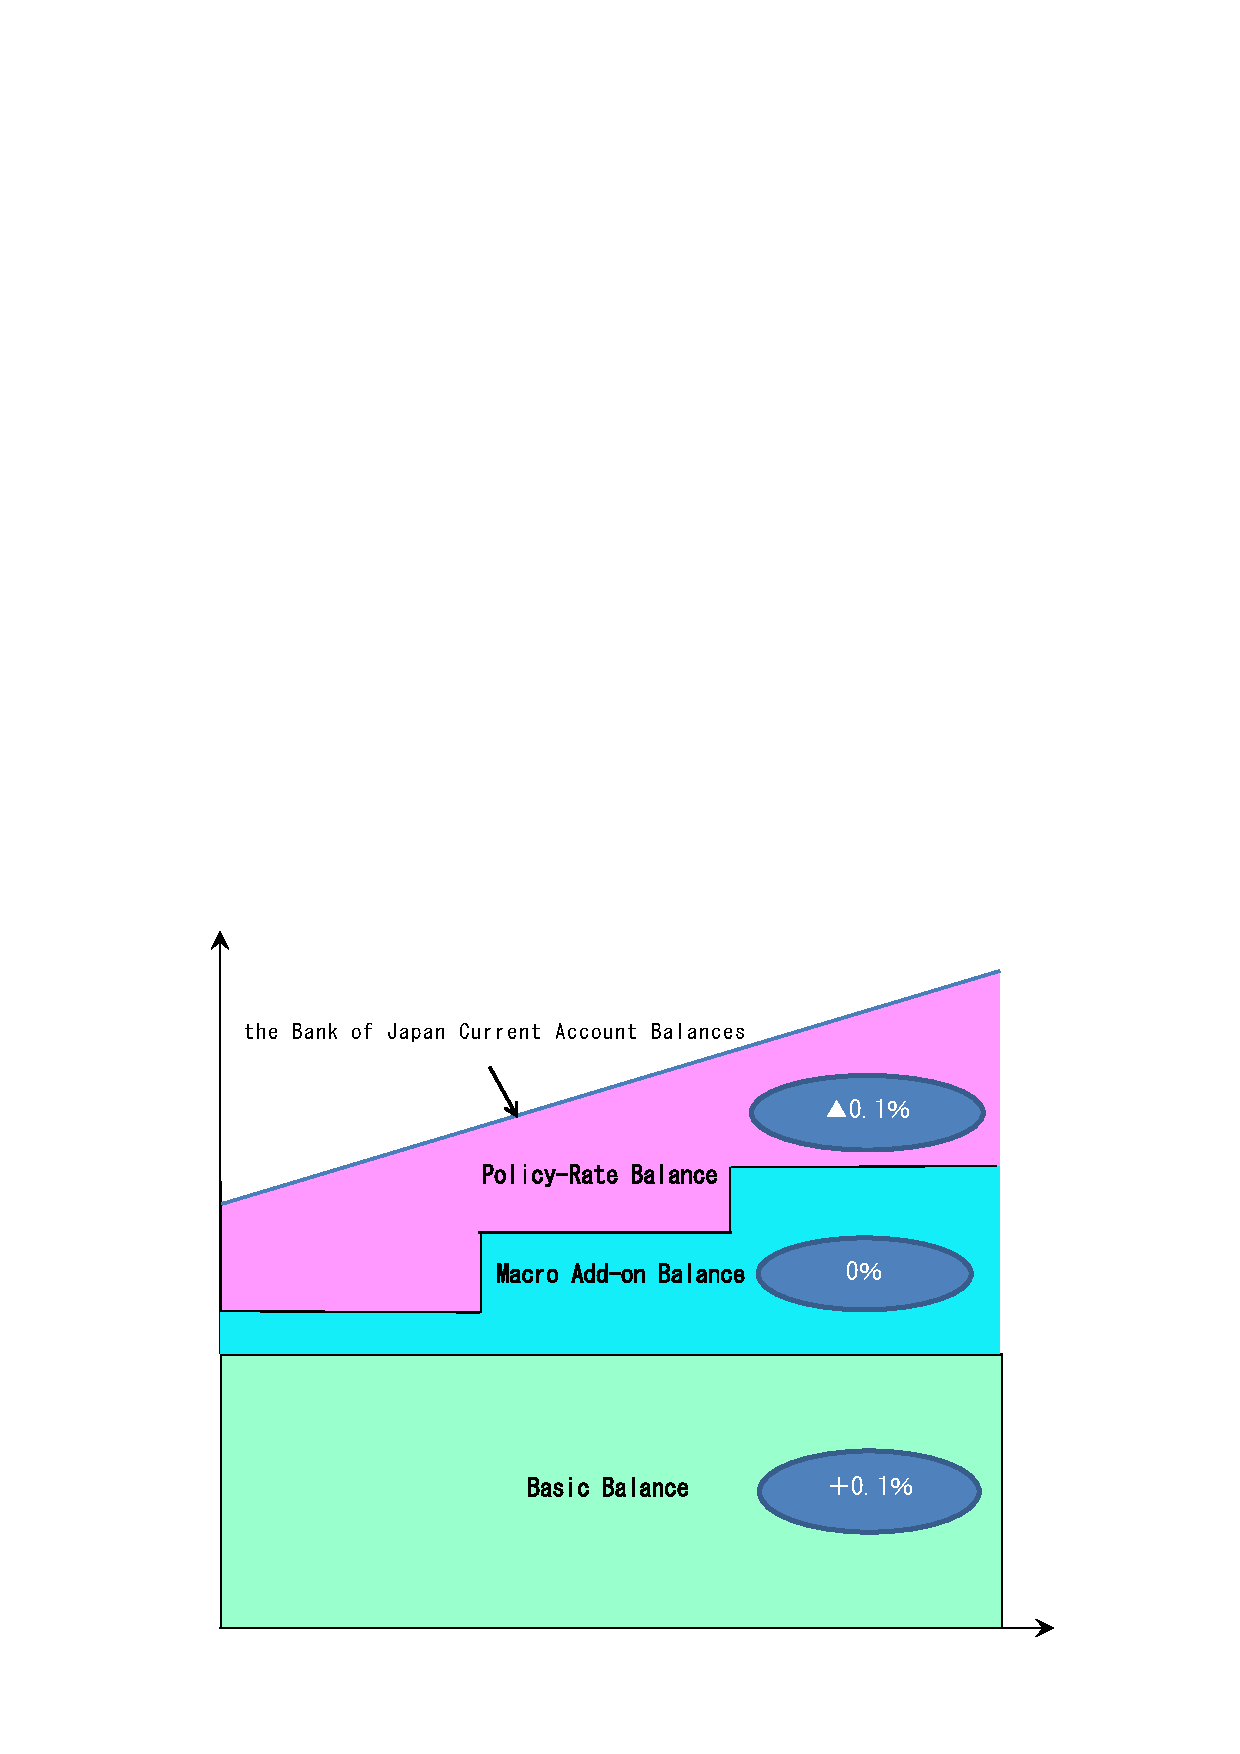
\includegraphics[width=17cm]{currentaccount.pdf}

    Compiled from the Bank of Japan documents on January 29, 2016.
\end{figure}

\newpage
\subsection{Effects of monetary easing policies in Europe}

There is a previous study by Pazicky [2018] that analyzed the effect of monetary policy on the inflation rate using a structural VAR model with Cholesky decomposition similarly in recent European data.
The study suggests that the effectiveness of monetary easing policy works on the economy in the long run due to the policy duration effect, which is mainly due to the decline in long-term interest rates.

Other previous studies that have analyzed the impact on financial markets include Fratzscher et al. [2014], Eser and Schwaab [2016], and Meszaros and Kiss [2020].
First, Fratzscher et al. [2014] is one of the first papers to quantify the impact of monetary policy in Europe, using panel data and a VAR model to analyze the impact on asset prices.
It concludes that while the SMP increased asset prices in the euro area, there was no portfolio rebalancing effect.
The paper also discusses the spillover effects on global stock markets.
Eser and Schwaab [2016] analyzed the impact of the SMP on long-term interest rates in the euro area and concluded that the introduction of the SMP reduced the risk premium on government bonds in the target countries, which had the effect of lowering long-term interest rates in both the short and long run.
The announcement of the start of SMPs was also considered to have had a significant effect.

Meszaros and Kiss [2020] analyze the effects of the ECB's monetary easing after the Lehman shock on government bond yields, stock indexes, and exchange rates, as well as their spillover channels.
It concludes that the portfolio rebalancing effect was due to changes in securities, foreign exchange reserves, and lending, which led to a decline in government bond yields and a depreciation of the local currency.
It is also concluded that this has had an effect on stock prices through various other channels.

As described above, as for the spillover channels of monetary policy in Europe, there are both positive and skeptical previous studies on the portfolio rebalancing effect, but most of them are positive about the decline in long-term interest rates.
Thus, many previous studies suggest that the policy duration effect works in Europe, where the ECB has cut the deposit rate multiple times, reducing the market's prediction of future short-term interest rates.

Demir [2014] analyzed the impact of monetary policy on the exchange rate and found a significant impact, but suggested that the quantitative impact was small.
Haitsma et al. [2016] concludes that it has a positive impact on the stock index, Eurostoxx 50 index (STOXX50), especially for value stocks.

\newpage

\section{Analysis method}

\subsection{Structural VAR Model}

In the analysis of this paper, the structural VAR model with Cholesky decomposition used in Honda et al. (2013) and Harada and Masushima (2009) is used.
The VAR model is widely used by central banks around the world and can model the effects between the same point in time.

In this paper, six endogenous variables are used to analyze the impact of monetary easing policies on inflation rates, financial markets and foreign exchange markets.

The period of analysis in this paper is from 2009, after the Lehman Shock, to the end of 2019, when data for all variables used were obtained.
However, during this sample period, Japan implemented a consumption tax hike in April 2014 (from 5\% to 8\%).
Therefore, in order to take this effect into account in the estimation of the model, a dummy variable for the consumption tax hike was added as an exogenous variable only for the analysis with Japanese data.
In addition, the consumption tax was increased in October 2019 (from 8\% to 10\%).
However, the impact of the tax hike is not expected to be significant due to the maintenance of the current 8\% tax rate on food products (excluding restaurants and alcoholic beverages) and home delivery newspaper subscriptions, as well as the "cashless point reduction project" implemented by the Ministry of Economy, Trade and Industry (METI) in Japan.

In the estimation of the structural VAR model in this paper, the level data is used without taking the factorial for all variables. This will be discussed in Section 3 of this chapter.

The standard VAR model cannot identify structural confounding terms from the results obtained from its analysis, which may make policy interpretation of the analysis results difficult when contemporaneous relationships among variables are considered.
However, since financial variables such as interest rates are expected to show a quick response to financial shocks within one day, this paper uses a structural VAR model with Cholesky decomposition that can take into account contemporaneous relationships among variables.

In the structural VAR model using Cholesky decomposition, the coefficient matrix $A_0$ is incorporated into the model to take into account the relationship between the same time points.
In this section, a model with the following short-term constraints is assumed.

\begin{equation}
    \label{eq1}
    A_{0} y_{t} = \alpha + \sum_{k=1}^{n} B_{k} y_{t-k} + \varepsilon_t
\end{equation}

$y_t$ is a $m$-dimensional vector representing the endogenous variables, $n$ is the lag of the endogenous variables, $\varepsilon$ is a $m$-dimensional vector representing the structural shocks, $\alpha$ is a constant term, and $A_0$, $B_0$ through $B_k$ are $m\times m$ square matrices.

Since the above structural VAR model cannot be estimated directly, the inverse of $A_0$ is multiplied on both sides.

\begin{equation}
    \begin{split}
        \label{eq2}
        y_t =A_0^{-1} \alpha + \sum_{k=1}^{n} C_{k} y_{t-k} +e_t \\
        (C_k = (A_0^{-1})\times B_k, \quad e_{t} = A_0^{-1} \varepsilon_t)
    \end{split}
\end{equation}

Harada and Masushima [2009] impose the constraint that $A_0^{-1}$ is a lower triangular matrix as in equation (\ref{eq3}).
Under this condition, the endogenous variables in the $s$th row $(0 < s \leq m)$ of $y_t$ are affected by the structural shocks in the endogenous variables from the first row to the $s$th row, but not in the endogenous variables from the $s + 1$th row onwards.
In addition, since the results differ depending on the order of the variables, it is necessary to arrange the variables so that the variables with high exogeneity are on top of the vector.
In this paper, in order to analyze how monetary policy variables, which will be discussed later, affect price inflation, we arranged and analyzed monetary policy variables, financial variables such as stock prices, and price indexes in this order.

\begin{equation}
    \label{eq3}
    A_0^{-1} = \left[
        \begin{array} {cccc}
            x      & 0      & \ldots & 0      \\
            \vdots & \ddots & \ddots & \vdots \\
            \vdots & \      & \ddots & 0      \\
            x      & \ldots & \ldots & x
        \end{array}
        \right]
\end{equation}

The lag in this VAR model is set to 1 for Japan and 2 for Europe, as selected by the Akaike's Information Criterion (AIC).

\subsection{Dummy variables and multiple regression equations}

In this paper, in addition to the analysis using the structural VAR model described above, the multiple regression analysis using dummy variables was conducted to analyze the effect of the Bank of Japan's announcement on prices.

In the structural VAR model, policy dummy variables can be incorporated into the model as exogenous variables, but this makes it difficult to measure effects of announcements of commitment to the inflation target.
Therefore, in this paper, this effect is measured by conducting a multiple regression analysis with policy dummy variables as explanatory variables.
This policy dummy variable takes the date of the announcement of the commitment to the price target as the policy start date, and takes the value 0 before and 1 after.
This enables it to take into account changes caused by a change in the central bank's policy.

On the other hand, as mentioned earlier, the ECB has not changed its inflation target since 2003, and this analysis was not conducted for the European data because it was not possible to analyze the impact on inflation during the period of monetary easing policy.

Therefore, the following multiple regression equation was used, with the price index as the objective variable and the policy dummy variable as the explanatory variable in addition to the financial variables similar to those used in the other structural VARs, excluding the monetary base.
As in the structural VAR model described above, in order to take into account the impact of the consumption tax hike, a consumption tax hike dummy variable was added to the explanatory variables, bringing the total number of explanatory variables to six.

\begin{equation}
    \label{eq4}
    \begin{gathered}
        y_i = \beta_0 + \sum_{j=1}^k \beta_j X_{ij} + \varepsilon_i \\
        i=1,2,...n : \mathrm{Index \: of \: the \: statistical \: observation \: value}\\
        j=1,2,...k : \mathrm{Number \: of \: explanatory \: variables}\\
        % y_i: 消費者物価指数   X_1: 短期金利 X_2: 長期金利\\
        % X_3: 為替レート X_4: 株価指数 X_5: 政策ダミー変数 X_6: 消費増税ダミー変数
    \end{gathered}
\end{equation}

In this expression, $y_i$ is the dependent variable, $\beta_0$ is the intercept of the model, $X_ij$ is the $j$th explanatory variable of the model ($j$= 1 to k), and $\varepsilon_i$ is the error term of the stochastic error model with zero expectation and variance $\sigma^2$.

Expressing this equation as a matrix equation gives the following equation.

\begin{equation}
    \label{eq5}
    \left[
        \begin{array} {c}
            y_1    \\
            y_2    \\
            \vdots \\
            y_n    \\
        \end{array}
        \right]
    =
    \left[
        \begin{array} {c}
            1,x_{11},x_{21},\cdots x_{k1}                                         \\
            1,x_{12},x_{22},\cdots x_{k2}                                         \\
            \vdots \hspace{20pt} \vdots \hspace{20pt} \vdots \hspace{20pt} \vdots \\
            1,x_{1n},x_{2n},\cdots x_{kn}                                         \\
        \end{array}
        \right]
    \cdot
    \left[
        \begin{array} {c}
            \beta_0 \\
            \beta_1 \\
            \beta_2 \\
            \vdots  \\
            \beta_k \\
        \end{array}
        \right]
    +
    \left[
        \begin{array} {c}
            \varepsilon_1 \\
            \varepsilon_2 \\
            \vdots        \\
            \varepsilon_n \\
        \end{array}
        \right]
\end{equation}

This equation can be simplified to the following equation.

\begin{equation}
    \label{eq6}
    Y = X B + E
\end{equation}

Using this equation, calculate the estimator of $B$.

\begin{equation}
    \label{eq7}
    \hat{B}=(X^T \cdot X)^{-1} \cdot X^T \cdot Y
\end{equation}

\newpage

\subsection{Problems in the analysis}

In the structural VAR model using Cholesky decomposition, the order of the variables is important, and it is known that different results will be obtained if the order changes.
This is because the earlier the order of the variables, the greater the impact of shocks on the other variables.
Therefore, the exogeneity of the variables needs to be carefully examined.
In the analysis of this paper, we have tried to identify the appropriate order by analyzing several sets of variables in different orders.
This paper presents the results of the analysis of the order of the variables considered to be most appropriate.

The reason why we used level data instead of factorial data for all variables in the estimation of the structural VAR model is that it is known that the estimators of the structural VAR model are consistent even if non-stationary variables are included in the estimation of the reduced VAR model.
In Teruyama (2001), it is noted that the main focus of prospective papers on the analysis of monetary policy using VAR models is on the estimation method as is, even when non-stationary series are included in the level term.
This relies on Sims et al. (1990) that the level estimators are consistent even when non-stationary variables are included.
Although the confidence interval of the impulse response function is not always appropriate when non-stationary variables are included, it is included in this paper for reference.

Many previous studies have also focused on the expected inflation rate and the real interest rate as the spillover channels of monetary easing policies.
The real interest rate is obtained by subtracting the expected rate of inflation from the nominal interest rate, but the expected rate of inflation data published by the International Monetary Fund (IMF) are annual data, so it is difficult to use them in the analysis of this paper.
Therefore, to deal with this problem, this paper uses stock prices and exchange rates, which are considered to be affected by the expected inflation rate and real interest rates, as alternative financial variables.

Based on the above analytical approach, this paper analyzes the relationship between monetary policy and price inflation, obtains robustness, and attempts to identify spillover channels.

\newpage

\section{Details of the data used}

In this paper, the sample period for the structural VAR model is monthly data from January 2009 to December 2019.
The reason for this is to analyze the effects of monetary policy on Japan and Europe after the Lehman Shock.
And, the reason why the data are monthly is that the ECB publishes macroeconomic data on a monthly basis.
In contrast, the Bank of Japan publishes data on a daily basis, but in order to match the sample size with the European data, the Japanese data are also used on a monthly basis.
The variables are six each: $JMB$, $JSTOCK$, $JLIBOR$, $JBOND$, $USDJPY$, and $JCPI$ for Japanese data, and $EMB$, $ESTOCK$, $ELIBOR$, $EBOND$, $USDEUR$, and $EHICP$ for European data.
The consumption tax hike dummy ($TAXDUMMY$), which was used as an exogenous variable only in the VAR analysis for the Japanese data, is a dummy variable that is set to 0 before April 2014 and 1 after.

This paper uses the monetary base (base money) as an indicator of quantitative and qualitative monetary easing as a monetary policy variable ($JMB, EMB$).
Although the money stock and the Bank of Japan's current account balance were also considered as other candidates for policy variables, they are not appropriate as monetary policy variables because the impact of monetary easing on the money stock is limited.
Since the impact of cash in circulation on price inflation is not considered to be small even for the BOJ current account balance, we adopted the monetary base, which is the sum of the BOJ current account balance and cash in circulation.

As the remaining financial market variables, the Nikkei 225 and the Euro Stoxx 50 were used as stock market indices in $JSTOCK$ and $ESTOCK$.
For interest rates, $JLIBOR$ and $ELIBOR$ are the 3-month yen-based and 3-month euro-based rates of the London Interbank Offered Rate (LIBOR), respectively, as short-term interest rate indices, and $JBOND$ and $EBOND$ are the 10-year yields on Japanese government bonds and 10-year yields on German-listed federal securities, respectively, as long-term interest rate indices.
In addition, the exchange rate is added as a variable because it is thought to have an impact on price increases through import prices.
In $USDJPY$, the spot rate between the dollar and the yen in the Tokyo market published by the Bank of Japan is used as an indicator of the foreign exchange market, and in $USDEUR$, the foreign exchange reference rate between the dollar and the euro published by the ECB is used.
The reason for using the dollar reference rate for both the Japanese and European data is that the U.S. Federal Reserve has not yet introduced negative interest rates, and the impact of monetary easing policies on exchange rates is believed to be smaller than for both the Bank of Japan and the ECB.
All values are based on closing prices.

As an index of price changes to measure the effects of the policy ($JCPI$), the Consumer Price Index excluding fresh food and energy (core core CPI) was used.
The reason why the index excluding fresh food and energy is used is that the price fluctuations of fresh food are large, and the price trend of energy cannot be captured because of the sharp decline in the price of crude oil today.
The monthly data released by the Ministry of Internal Affairs and Communications (MIC) in Japan was used as the data for the core core CPI.

As a similar index of price changes in Europe ($EHICP$), the EU benchmark consumer price index excluding food and energy is used.
This index is based on the Maastricht Treaty harmonized standards for the EU member states, and is considered to be the most similar to the core core CPI as a price index for Europe published by the ECB.

Both $JCPI$ and $EHICP$ are converted into indices with 2015 as the base year and the average of the data for the year 2015 as 100.

The details and sources of these data are shown in the table below. Note that the natural logarithm is taken for $JMB$, $EMB$, $JSTOCK$, $ESTOCK$, $USDJPY$, $JCPI$, and $EHICP$.

In the multiple regression analysis, we used the same data set ($JSTOCK$, $JLIBOR$, $JBOND$, $USDJPY$, and $TAXDUMMY$) excluding the policy variable ($JMB$).
In addition, a policy dummy variable $ITDUMMY$ is set to 0 before and 1 after January 2013, when the price stability target of 2 percent was introduced.
$OSDUMMY$, a policy dummy variable that is set to 0 before and 1 after September 2016, when the "Overshooting Commitment" was issued.

%%変数のリスト
\newpage
\begin{table}[H]
    \centering
    \caption{Variables for Japan used in this paper}
    \vspace{10pt}
    \begin{threeparttable}
        \begin{tabular}{ccc} \toprule[0.5pt]\toprule[0.5pt]
            Variable name & Definition                                                           & Source \\ \midrule[0.5pt]
            $JMB$         & Monetary base (100 million yen)                                      & BOJ    \\
            $JSTOCK$      & Nikkei Stock Average Index (Nikkei225)                               & Nikkei \\
            $JLIBOR$      & London Interbank Offered Rate (LIBOR, 3-month) (Yen-based) (\%)      & FRED   \\
            $JBOND$       & 10-year yield on Japanese government bond (\%)                       & MOF    \\
            $USDJPY$      & Tokyo market dollar/yen spot rate (Yen/\$)                           & BOJ    \\
            $JCPI$        & Consumer Price Index excluding fresh food and energy (Core core CPI) & MIC    \\
            $TAXDUMMY$    & Tax hike dummy variable with 0 for before April 2014 and 1 for after &        \\
            $ITDUMMY$     & Policy dummy variable with 0 before January 2013 and 1 after         &        \\
            $OSDUMMY$     & Policy dummy variable with 0 before September 2016 and 1 after       &        \\
            \bottomrule[0.5pt]\bottomrule[0.5pt]
        \end{tabular}
        \vspace{10pt}
        \begin{tablenotes}\footnotesize
            \item[1] All data are monthly data.
            \item[2] The closing price is used for all time series data.
            \item[3] $JMB$, $JSTOCK$, $USDJPY$, and $JCPI$ are taken the natural logarithm.
        \end{tablenotes}
    \end{threeparttable}
\end{table}

\vspace{80pt}

\begin{table}[H]
    \centering
    \caption{Variables for Europe used in this paper}
    \vspace{10pt}
    \begin{threeparttable}
        \begin{tabular}{ccc} \toprule[0.5pt]\toprule[0.5pt]
            Variable name & Definition                                                       & Source     \\ \midrule[0.5pt]
            $EMB$         & ECB Base Money (million euros)                                   & ECB        \\
            $ESTOCK$      & Euro Stoxx 50 Index                                              & ECB        \\
            $ELIBOR$      & London Interbank Offered Rate (LIBOR, 3-month) (Euro-based) (\%) & FRED       \\
            $EBOND$       & 10-year yield on German listed federal securities (\%)           & Bundesbank \\
            $USDEUR$      & ECB Reference Exchange Rate (\euro /\$)                          & ECB        \\
            $EHICP$       & Harmonised Index of Consumer Prices excluding food and energy    & ECB        \\
            \bottomrule[0.5pt]\bottomrule[0.5pt]
        \end{tabular}
        \vspace{10pt}
        \begin{tablenotes}\footnotesize
            \item[1] All data are monthly data.
            \item[2] The closing price is used for all time series data.
            \item[3] The $EMB$ is used to interpolate data using the cubic interpolation method for some missing data.
            \item[4] The $EHICP$ was seasonally adjusted using "X-12-ARIMA" since there were no seasonally adjusted data.
            \item[5] $EMB$, $ESTOCK$, and $EHICP$ are taken the natural logarithm.
        \end{tablenotes}
    \end{threeparttable}
\end{table}


%%変数の推移
\begin{figure}[!htbp]
    \centering
    \caption{Transition of each variable}
    \vspace{10pt}
    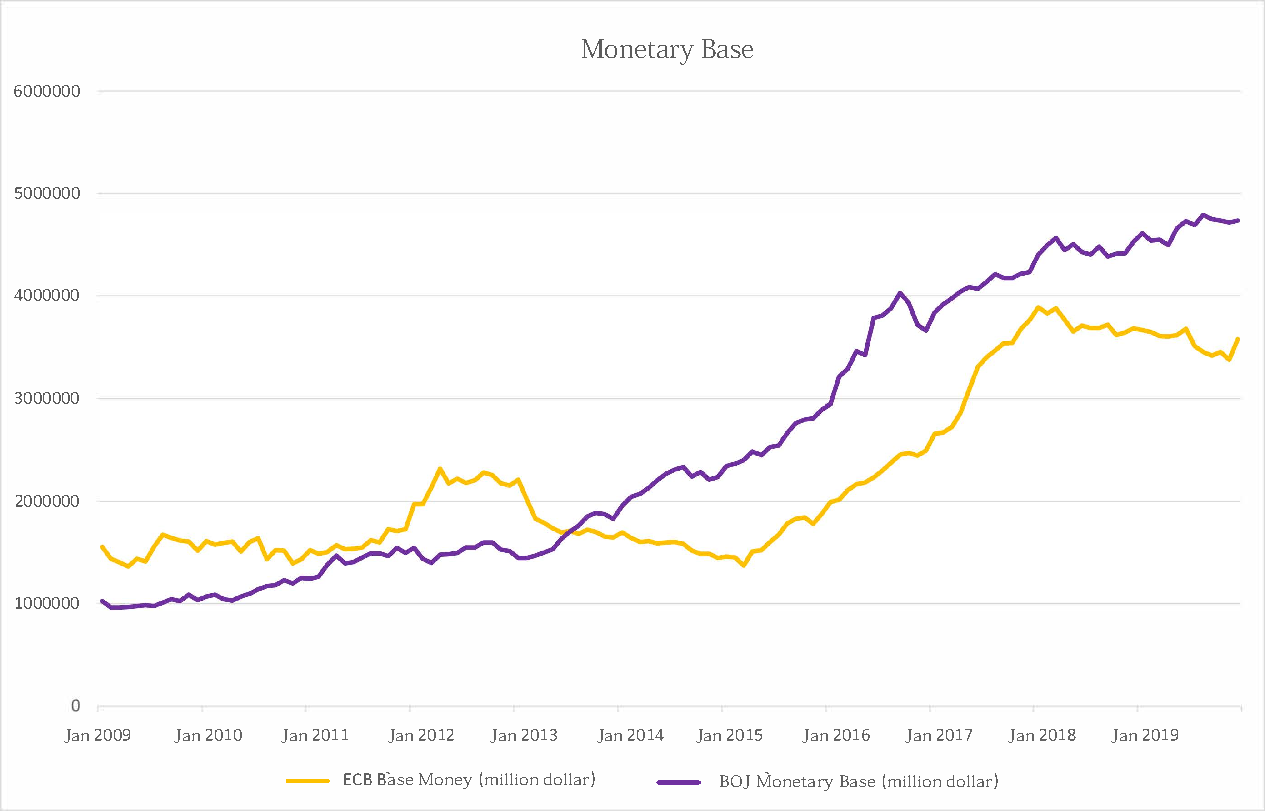
\includegraphics[width=16cm]{mbfix.pdf}
    \vspace{10pt}
    \begin{tablenotes}\footnotesize
        \item[1] The units were aligned using $USDJPY$ and $USDEUR$ for $JMB$ and $EMB$, respectively.
    \end{tablenotes}
    \vspace{10pt}
    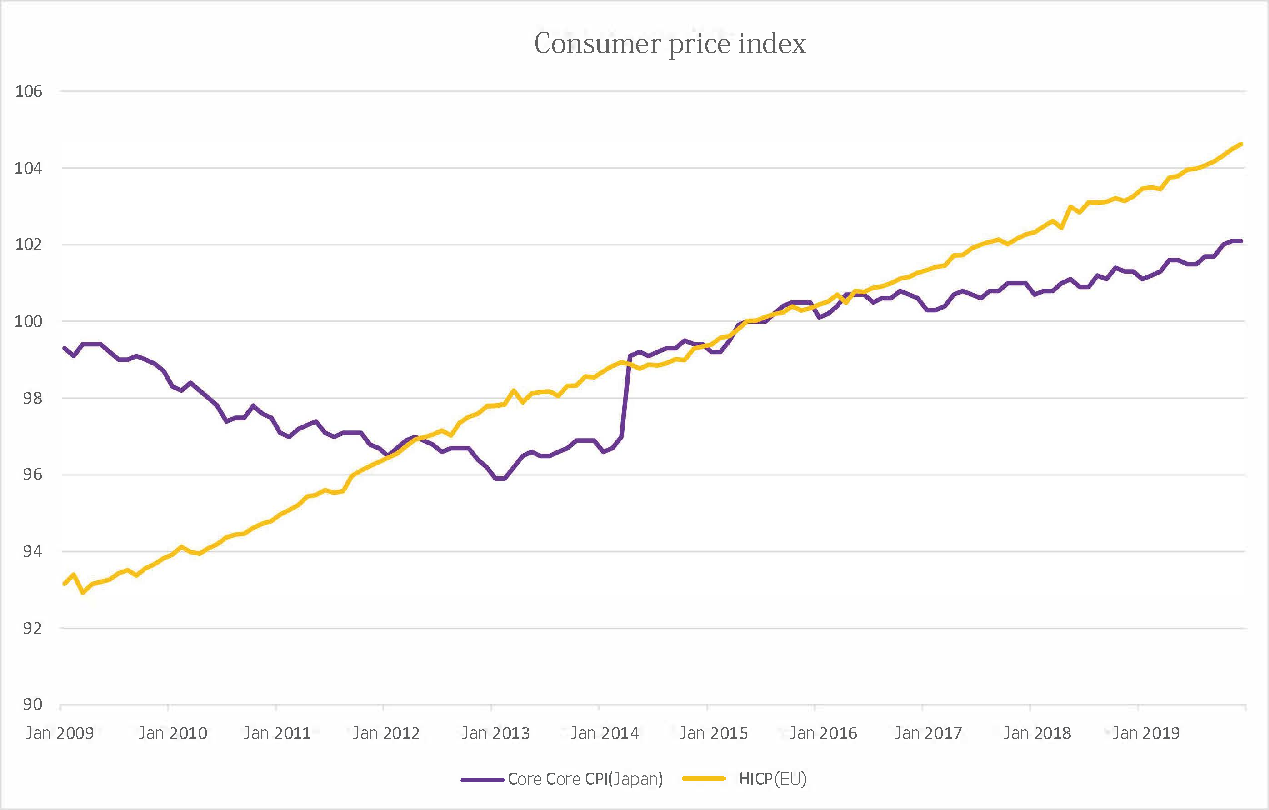
\includegraphics[width=16cm]{cpi09.pdf}
    \vspace{10pt}
    \begin{tablenotes}\footnotesize
        \item[1] Both $JCPI$ and $EHICP$ are indices with the one-year average of 2015 as 100.
    \end{tablenotes}
\end{figure}

\newpage
\begin{figure}[!htbp]
    \centering
    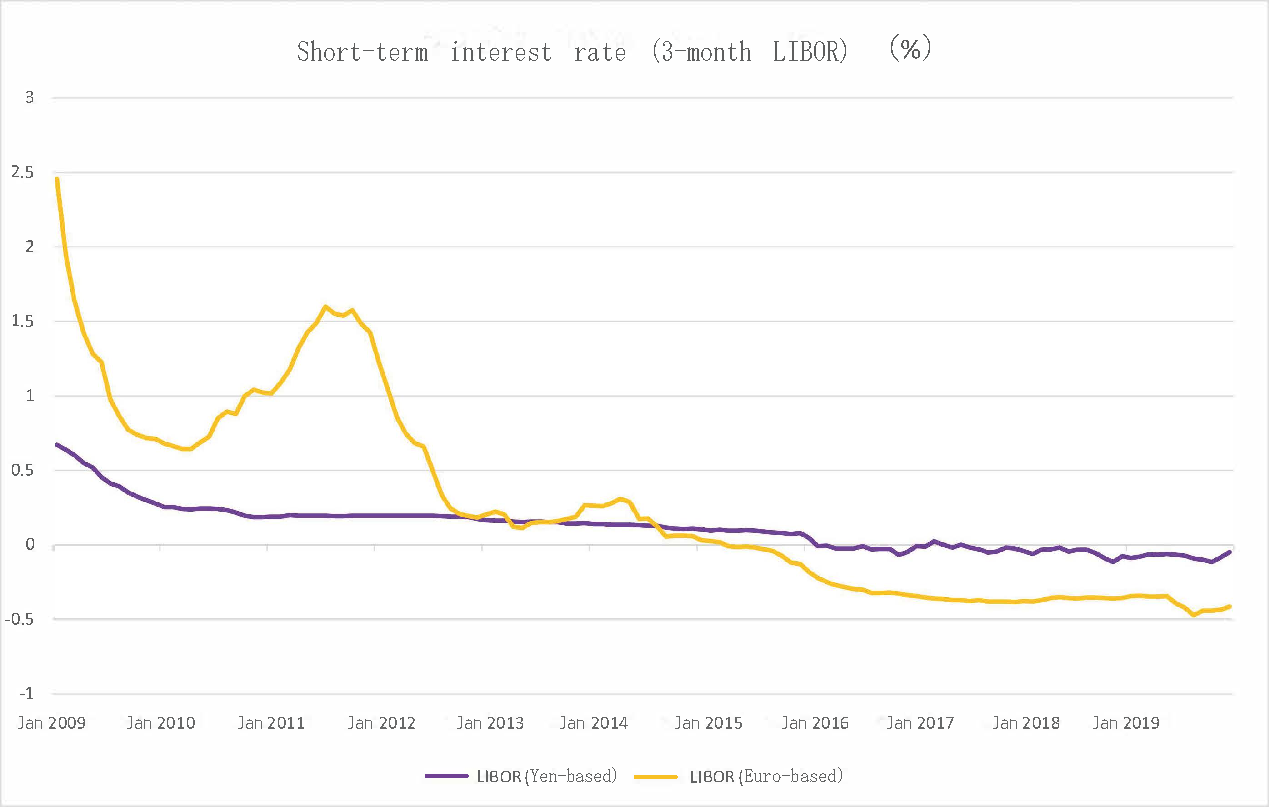
\includegraphics[width=16cm]{libor09.pdf}
\end{figure}
\begin{figure}[!htbp]
    \centering
    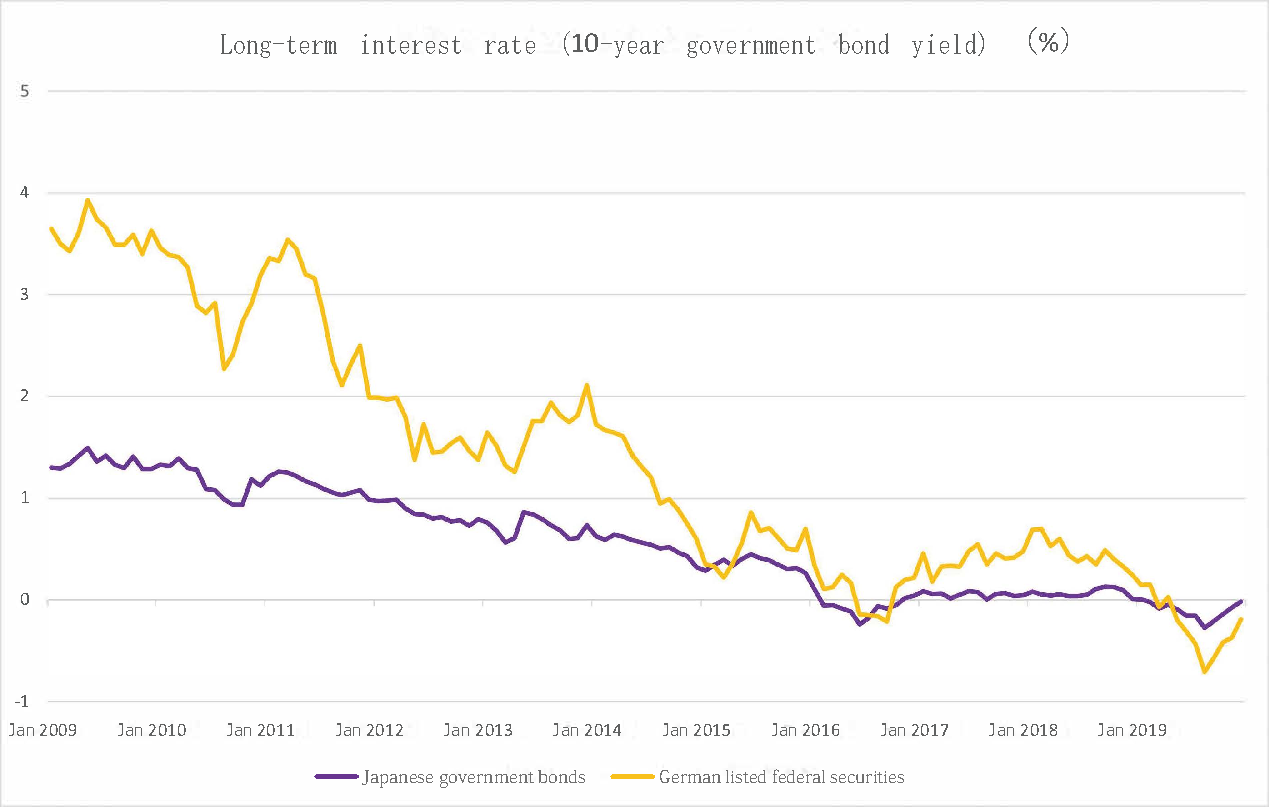
\includegraphics[width=16cm]{bond09.pdf}
\end{figure}
\newpage

\section{Results of the analysis}

\subsection{Cholesky Decomposition}

In this chapter, the estimation is carried out using a structural VAR model with Cholesky decomposition.
The order of exogeneity of the variables is $JMB$, $JLIBOR$, $JBOND$, $USDJPY$, $JSTOCK$, and $JCPI$ for the Japanese analysis, and $EMB$, $ELIBOR$, $EBOND$, $USDEUR$, $ESTOCK$, and $EHICP$ for the European analysis as well.
This order of variables was used in this order, but similar results were obtained with other possible orders.
Due to the inclusion of non-stationary variables in the model, it cannot be said that the estimated impulse response function is significant at the confidence interval.
However, in this estimation, it is assumed that this does not significantly affect the significance, and the assumed spillover effects are presented with reference to the 95\% confidence interval.

The cumulative impulse response of the VAR analysis is shown in the following figure.
The results of the analysis suggest that the following relationships exist in the Japanese data.

\begin{enumerate}
    \setlength{\leftskip}{30pt}
    \item The expansion of Japan's monetary base will raise the CPI.
    \item The expansion of Japan's monetary base will lower long-term interest rates.
    \item The expansion of Japan's monetary base will cause the yen to weaken and spill over to higher stock prices.
\end{enumerate}

As shown in result 1, the effect of monetary base expansion on raising the CPI seems certain.
In addition, the effect of monetary easing policies on lowering long-term interest rates, as shown in result 2, is consistent with previous studies such as Wright [2011].
The effect of monetary easing to weaken the yen and contribute to higher stock prices, as shown in result 3, is also a spillover effect of monetary easing, as confirmed by Honda et al. [2013].

The figure suggests that the depreciation of the yen and the rise in stock prices are spillover channels for the rise in the CPI, but it is difficult to say that the spillover channels could be identified from the cumulative impulse responses, which all show the direct impact on the CPI.
In addition, the decline in long-term interest rates was also assumed to be a spillover channel of the monetary easing policy, but the effect is not confirmed from this analysis.

\newpage
\begin{figure}[!htbp]
    \caption{Impulse response of the structural VAR model on Japanese data}
    \begin{center}
        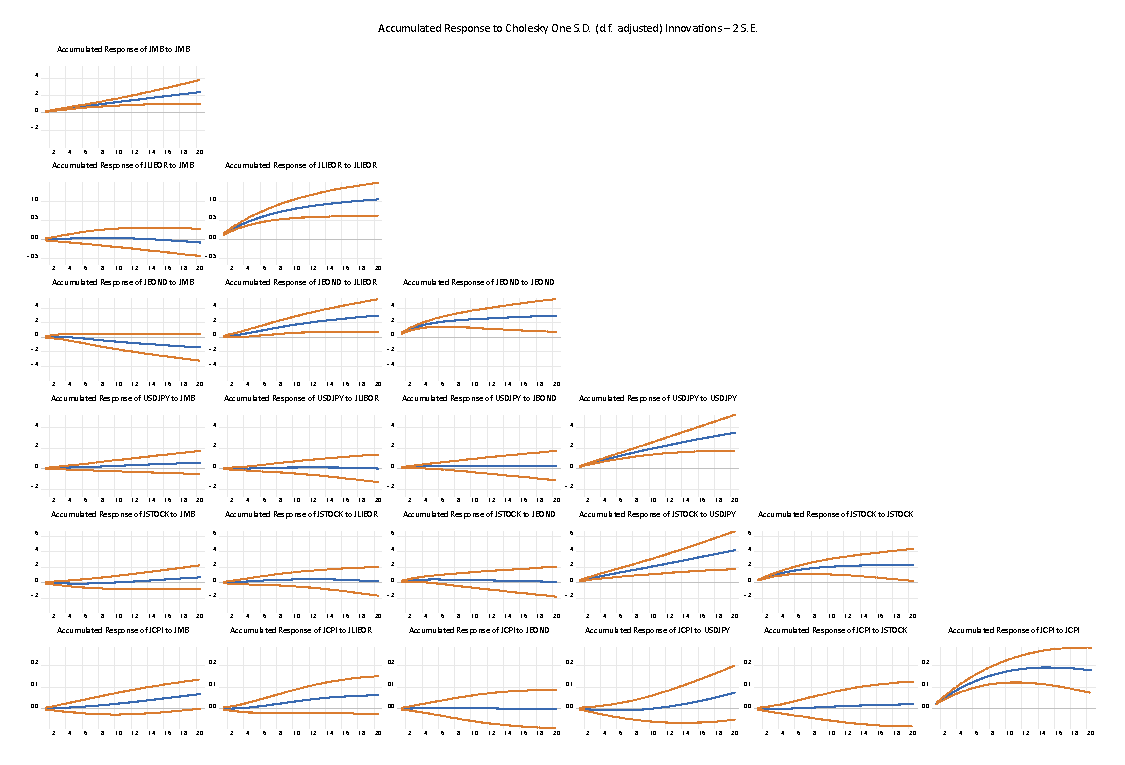
\includegraphics[width=18cm]{jimpulse.pdf}
    \end{center}
\end{figure}

\newpage

\begin{figure}[!htbp]
    \begin{minipage}{0.5\hsize}
        \caption{Impulse response of the long-term interest rate}
        \begin{center}
            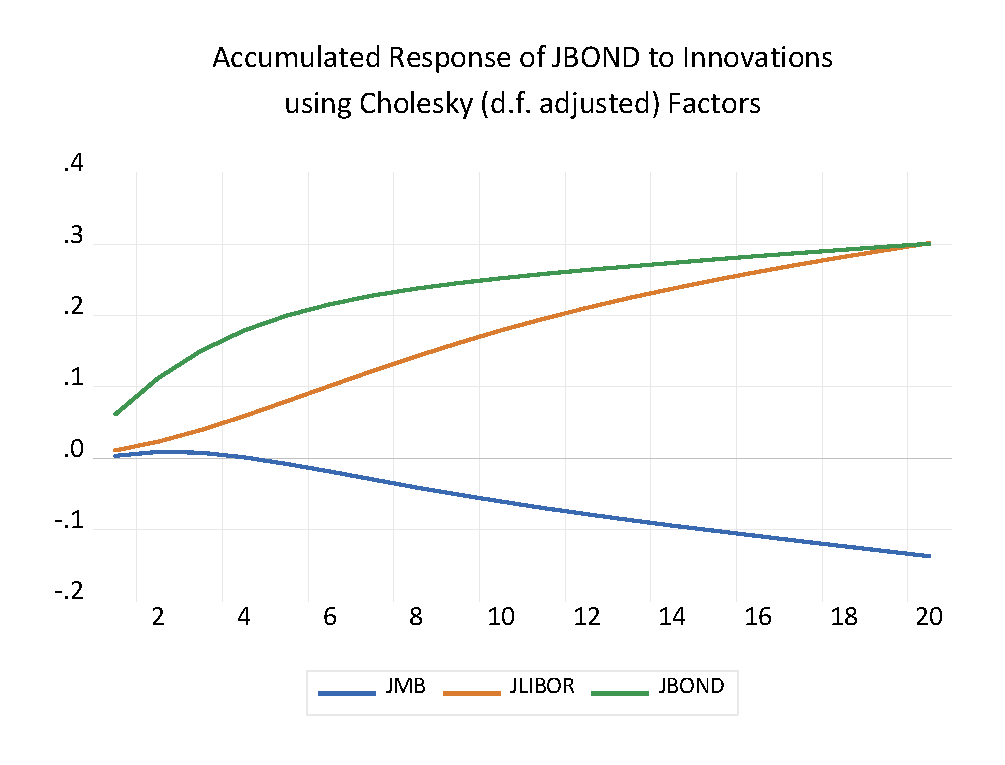
\includegraphics[width=9cm]{ijbond.pdf}
        \end{center}
    \end{minipage}
    \begin{minipage}{0.5\hsize}
        \caption{Impulse response of the exchange rate}
        \begin{center}
            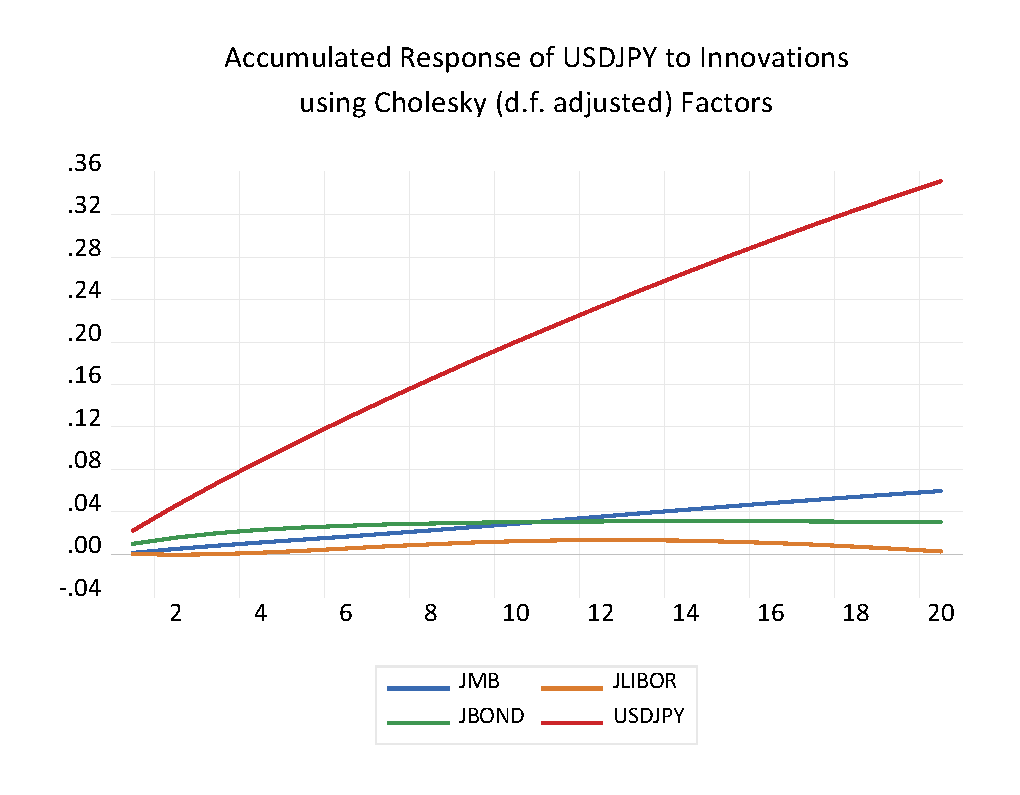
\includegraphics[width=9cm]{ijrate.pdf}
        \end{center}
    \end{minipage}
    \begin{minipage}{0.5\hsize}
        \caption{Impulse response of the stock price}
        \begin{center}
            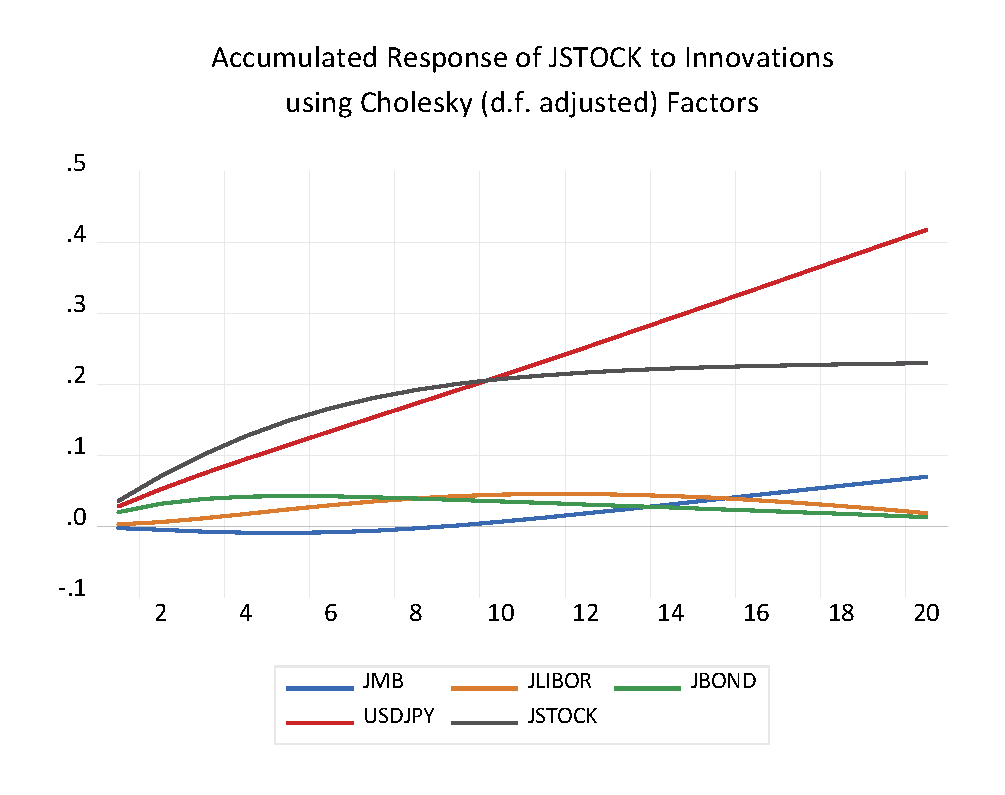
\includegraphics[width=9cm]{ijstock.pdf}
        \end{center}
    \end{minipage}
    \begin{minipage}{0.5\hsize}
        \caption{Impulse response of the core core CPI}
        \begin{center}
            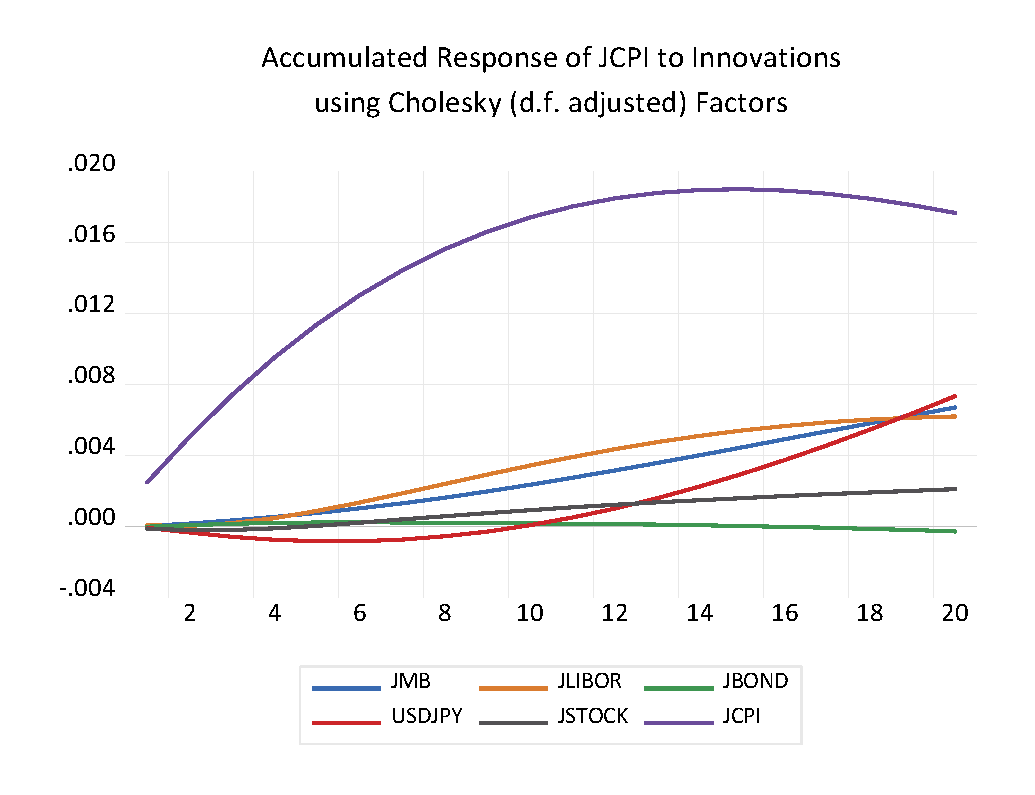
\includegraphics[width=9cm]{ijcpi.pdf}
        \end{center}
    \end{minipage}
\end{figure}

\newpage

Next, the analysis of the European data suggested that the following relationships exist.
The cumulative impulse response of the VAR analysis is shown in the following figure.

\begin{enumerate}
    \setlength{\leftskip}{30pt}
    \item The expansion of the monetary base in Europe will raise the HICP.
    \item The expansion of the monetary base in Europe will lower short-term interest rates and spill over to higher stock prices.。
    \item The expansion of the monetary base in Europe will cause the euro to weaken and spill over to higher stock prices.
    \item Higher stock prices in Europe will spill over to higher HICP.
\end{enumerate}

In Europe, as in Japan, monetary easing policies have been found to have a positive effect on the CPI by expanding the monetary base.
The same is true for the effect of monetary easing on stock prices by causing the depreciation of the local currency.
The cumulative impulse response also suggests that the depreciation of the local currency and the resulting rise in stock prices were likely to have affected inflation in Europe, and that this was a spillover channel of the monetary easing policy.

In addition, the effect of lowering the short-term interest rate and its spillover to stock prices is observed.
This is not observed in the Japanese data.
On the other hand, there was no decline in the long-term interest rate due to the policy duration effect identified in Pazicky [2018].

\newpage
\begin{figure}[!htbp]
    \centering
    \caption{Impulse response of the structural VAR model on European data}
    \vspace{10pt}
    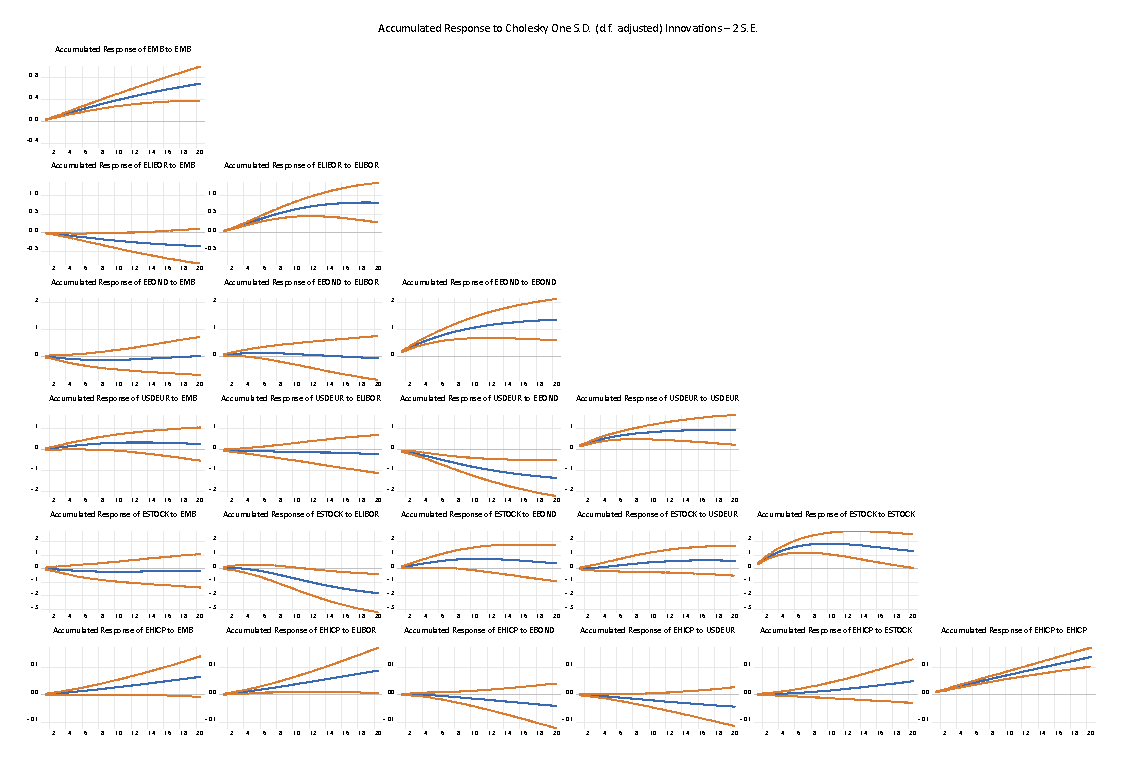
\includegraphics[width=18cm]{eimpulse.pdf}
\end{figure}

\newpage

\begin{figure}[!htbp]
    \begin{minipage}{0.5\hsize}
        \caption{Impulse response of the short-term interest rate}
        \begin{center}
            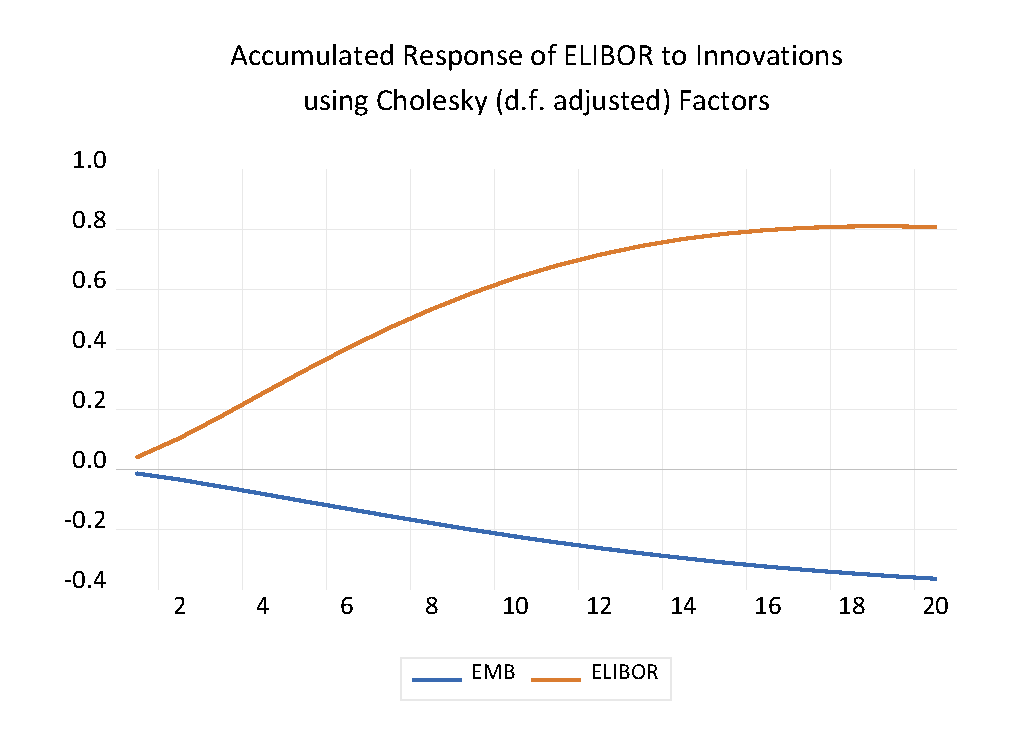
\includegraphics[width=9cm]{ielibor.pdf}
        \end{center}
    \end{minipage}
    \begin{minipage}{0.5\hsize}
        \caption{Impulse response of the exchange rate}
        \begin{center}
            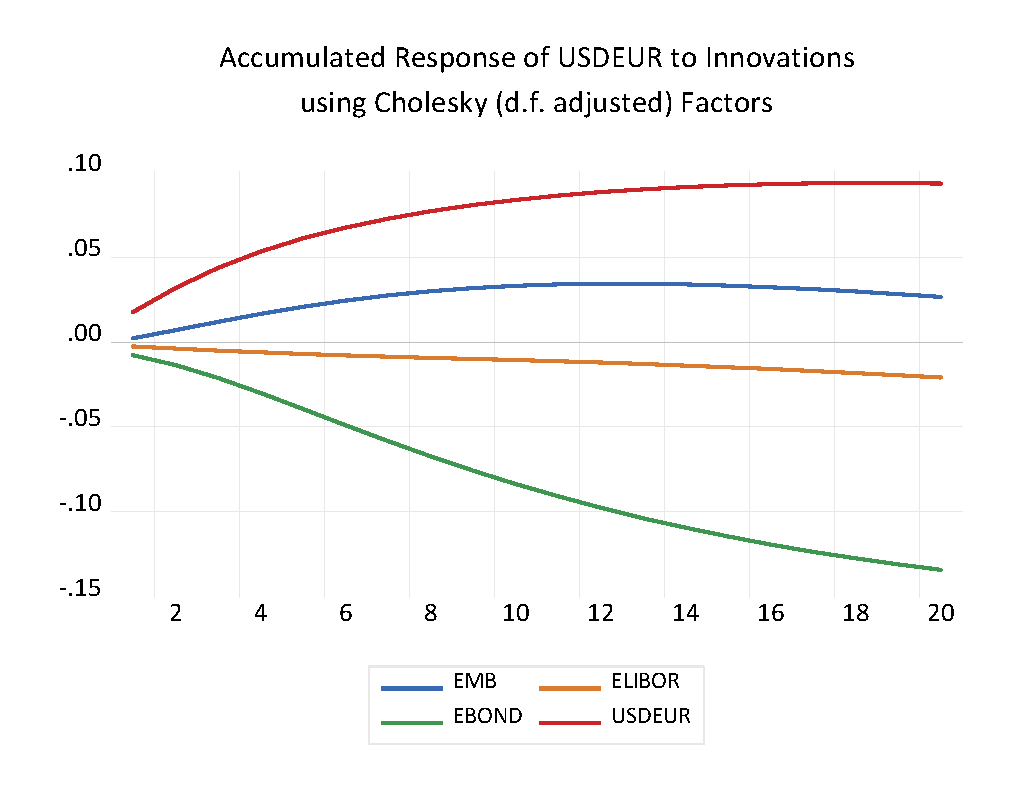
\includegraphics[width=9cm]{ierate.pdf}
        \end{center}
    \end{minipage}
    \begin{minipage}{0.5\hsize}
        \caption{Impulse response of the stock price}
        \begin{center}
            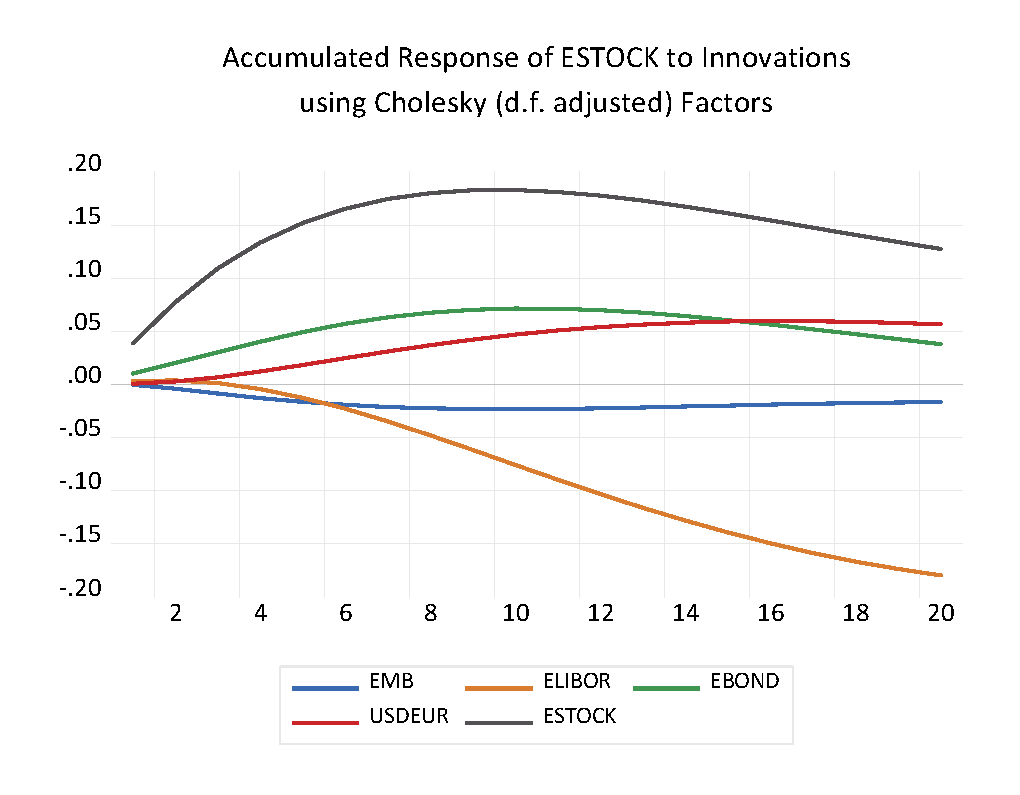
\includegraphics[width=9cm]{iestock.pdf}
        \end{center}
    \end{minipage}
    \begin{minipage}{0.5\hsize}
        \caption{Impulse response of the HICP}
        \begin{center}
            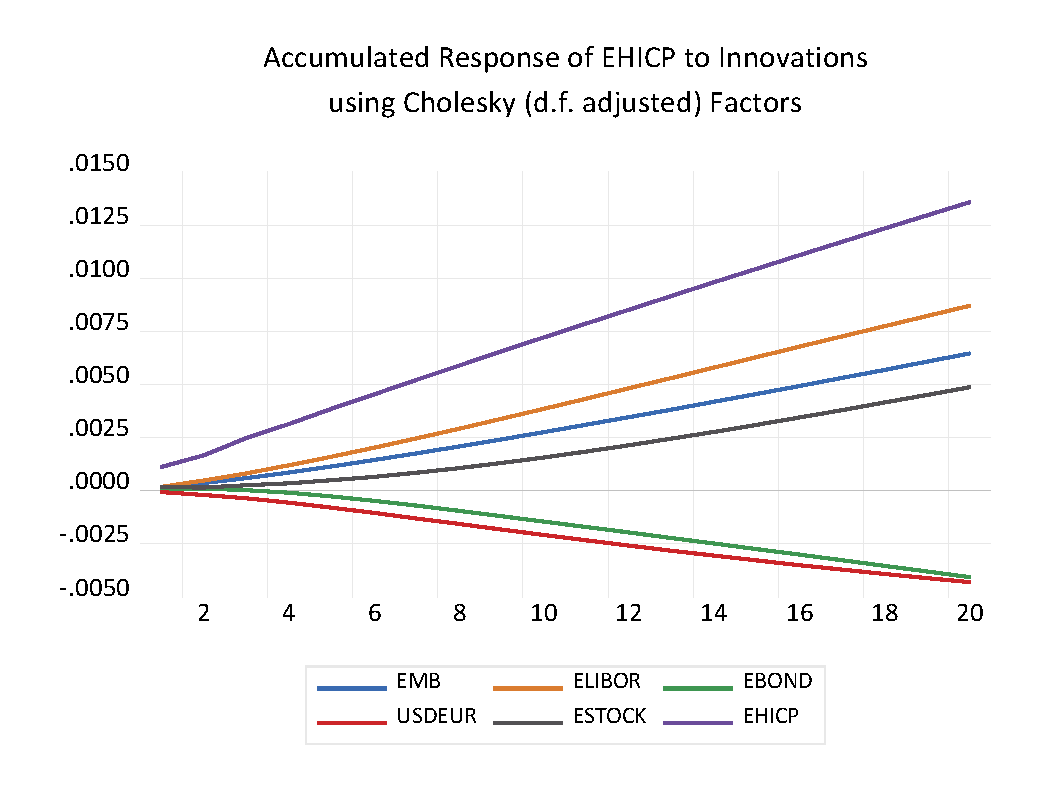
\includegraphics[width=9cm]{iehicp.pdf}
        \end{center}
    \end{minipage}
\end{figure}

\newpage
\subsection{Multiple regression analysis}

\end{document}